%\newpage


\appendix

\section{Further Examples}


A second example for the foreign-key optimization:


\begin{example}
Consider again Example~\ref{ex:ssb}:
\begin{verbatim}
SELECT   P.partcat, D.year, SUM(revenue)
FROM     Date D, Part P, LineOrder L
WHERE    D.datekey=L.datekey
AND      P.partkey=L.partkey
GROUP BY P.partcat, D.year;

+Date(datekey, year):
 (partcat: Part.partcat)
    m[partcat, year] += mD[datekey, partcat];
 (partkey: Part.partkey)
    mP[partkey, year] += mDP[datekey, partkey];
 mPL[datekey, year] += 1

+Part(partkey, partcat):
 (year: Date.year)
     m[partcat, year] += mP[partkey, year];
 (datekey: Date.datekey)
    mD[datekey, partcat] += mDP[datekey, partkey];
 mDL[partkey, partcat] += 1

+LineOrder(datekey, partkey, revenue):
 (partcat: Part.partcat, year: Date.year)
  m[partcat, year] += revenue
    * mPL[datekey, year] * mDL[partkey, partcat];
 (partcat: Part.partcat) mD[datekey, partcat] +=
    revenue * mDL[partkey, partcat];
 (year: Date.year) mP[partkey, year] +=
    revenue * mPL[datekey, year];
 mDP[datekey, partkey] += revenue;


on insert into Date (datekey, year) {
 mPL[datekey, year] += 1
}
on insert into Part (partkey, partcat) {
 mDL[partkey, partcat] += 1
}
on insert into LineOrder
           (datekey, partkey, revenue) {
  (partcat: Part.partcat, year: Date.year)
  m[partcat, year] += revenue
                    * mPL[datekey, year]
                    * mDL[partkey, partcat]
}
\end{verbatim}
\end{example}


%\section{Figures}


\begin{figure}
\begin{center}
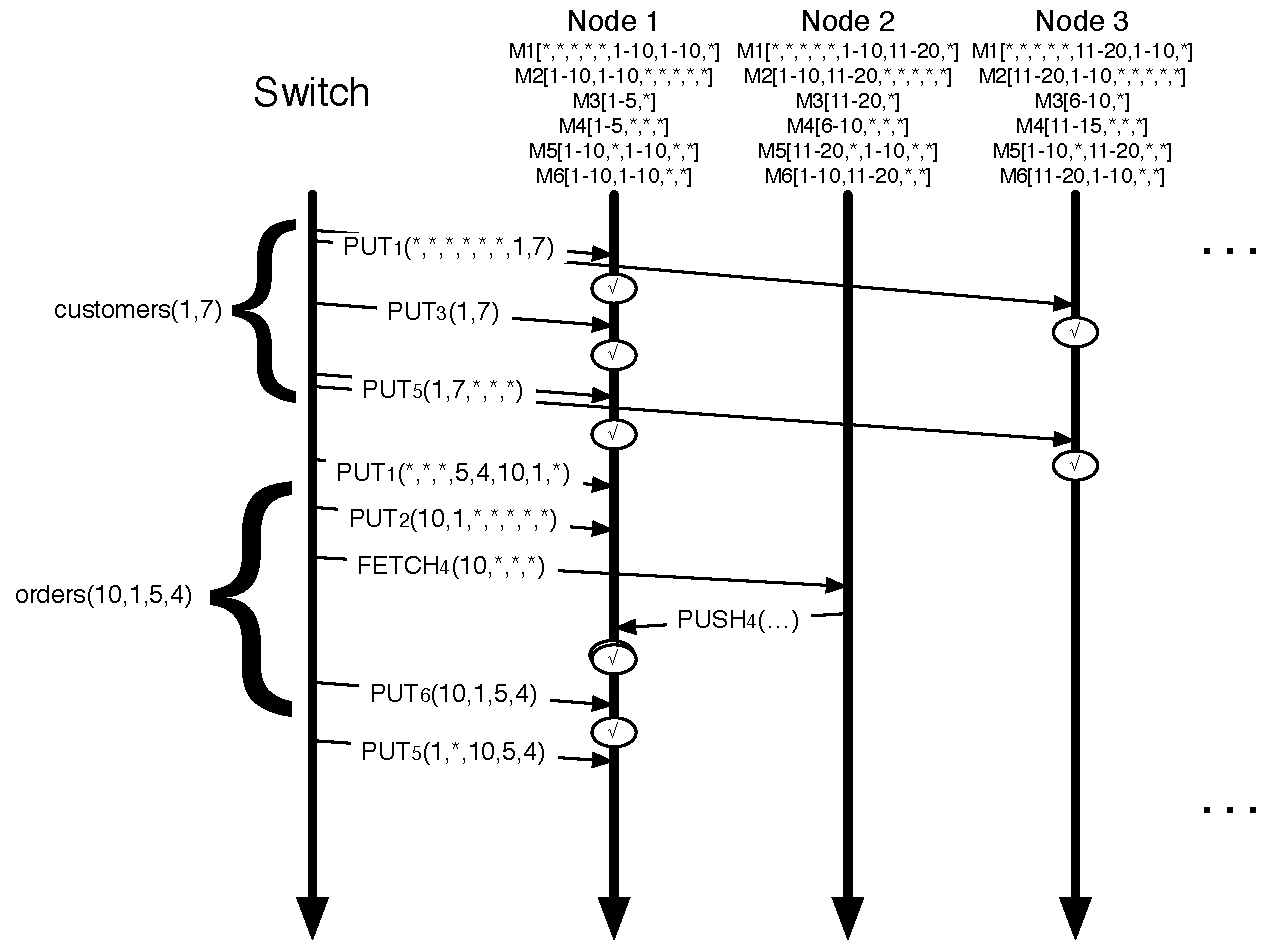
\includegraphics[width=3.5in]{images/MessageFlow.pdf}
\caption{Sequence diagram.}
\end{center}
\end{figure}

